\section{Stacking}

In this section we will talk about the white noise localization algorithm described in the paper "Direction of Arrival with One Microphone, a few LEGOs, and Non-Negative Matrix Factorization" \cite{dalia}. As stated in the title of the paper, this algorithm is described how to be used for one microphone in the paper so in order to be able to use it in this project we have to adapt it. The adaptation is done by stacking the different impulse responses of the different mics and use it as if it was a unique microphone. It is important to notice that this algorithm is done assuming an anechoic case (i.e. no echos, only the direct sound is taken in account).

\subsection{Description of the impulse response} \label{desc:impulse}

First of all, we would like to address how the impulse responses that we have look like. For the LEGO case we have 6 different microphones each having different impulse responses. These responses have a discretization of 180 different angles, each angle being 2 degrees apart from each other. And for each angle we get an impulse response in time domain for 160 units of time. For the KEMAR case we have 2 different microphones and their responses have a discretization of 360 different angles but for the sake of this project we will only select 180 different angles and again each angle will be 2 degrees apart so that the comparison with the LEGO case is fair. For the last case, the omnidirectional one, the responses that we will have are analytically computed assuming a far-field model and using the following function for omnidirectional sound \begin{math} H(w) = e^{-jw\tau} \end{math} with $\tau = \frac{d}{c}$, d is the distance between the source and the microphone and c is the speed of sound ($c = 343 \left[\frac{m}{s}\right]$). As we are assuming far field the distance between the source and the microphone is computed using the angle so the source would be at an hypothetical position $ \binom{cos(\theta)}{sin(\theta)}$ from the microphone if we want the sound coming from the $\theta$ angle. In the same way as for the other responses we will use 180 angles each 2 degrees apart for fairness.

\subsection{Description of the algorithm }

\subsubsection{Idea of the algorithm} \label{sect:idea}

As explained in section \ref{desc:impulse}, we will use 180 different angles. Meaning that the azimuth is discretized into 180 candidate source locations. In this description we will use D different angles to illustrate the algorithm, while keeping in mind that we have 180 angles in our case, so the locations could be $\Omega = \{\theta\textsubscript{1}, \theta\textsubscript{2}, \theta\textsubscript{3} ... \theta\textsubscript{D}\}$. We consider now the standard mixing model in time domain. Having L sources coming from the direction $\Theta = \{\theta\textsubscript{j}\}_{j\in J} ,$ the standard mixing model is 

\begin{equation}
    y(t) = \sum_{j\in J} s\textsubscript{j}(t)*h\textsubscript{j}(t) + e(t)
    \label{equ:time}
\end{equation}

where the parameters are; J the different sources, each source j $\in \{1, 2, 3 ... D\}$, |J| = L, * is the convolution, $s_j$ is the signal sent by the $j^{th}$ source, $h_j(t)$ is the impulse response corresponding to the angle $\theta_j$, y is the observed signal at the microphone corresponding to the impulse response h and e(t) is additive noise \cite{dalia}\cite{falSchro}. So, using the observed signal y, we want to find where the sources are, meaning we want to find the set $\Theta$. We can also compute the short-time Fourier transform to approximate the equation \ref{equ:time} in frequency domain. 

\begin{equation}
    Y(n,f) = \sum_{j \in J} S_j(n,f)H_j(f) + E(n,f),
\end{equation}

where f and n denotes the frequency and time indices \cite{dalia}\cite{falSchro}.

As stated in the introduction of this section, this algorithm is done by stacking the different impulse responses and observed signals so to be able to consider these stackings as a unique microphone and signal. For monaural localization if the source is always the same (for example a white noise source) then the localization is simple because each direction gives a different spectral signature, if the impulse responses uses scattering, and we can detect it by correlation. Of course, in reality, the source is never fixed but this idea helps for the algorithm and the approximation that we do.

So if the sources are white noise and we have the different transfer function $\{H_d\}^D_{d = 1}$ (i.e. the impulse responses) we can use the power spectral density (PSD) to approximate the direction(s) of arrival of the source(s) \cite{dalia}. For a white source the PSD is flat and scaled by its power meaning that 
\begin{equation}
    \mathbb{E}[|S_j|^2] = \sigma^2_j.
\end{equation}

And, when assuming that the noise has a zero mean, the PSD of the observed signal is 

\begin{equation}
    \mathbb{E}[|Y|^2] = \sum_{j \in J} \sigma^2_j |H_j|^2.
\end{equation}

So $\mathbb{E}[|Y|^2]$ belongs to a cone defined as 

\begin{equation}
    C_J = \{x : x = \sum_{j \in J} c_j |H_j|^2 , c_j > 0\},
\end{equation}

each cone $C_J$ corresponds to a different combination of the sources meaning that there is $\binom{D}{L}$ different cones as we have D directions and L sources \cite{dalia}. Knowing all that, the localization only becomes a simple approximation problem where we have to identify the closest cone 

\begin{equation}
    \hat J = arg min_Jdist(\mathbb{\hat E}[|Y|^2], C_J),
\end{equation}

where $\mathbb{\hat E}[|Y|^2]$ corresponds to the expectation $\mathbb{E}[|Y|^2]$ computed empirically using the observed measurements. This estimation of the angles works when the different cones are distinct meaning that if $C_{J_1} = C_{J_2}$ then  $J_1 = J_2$ \cite{dalia}. And this will more likely hold when the different $H_j$ are diverse, this is the reason why scattering helps with monaural localization. 

\begin{figure}[h]
\centering
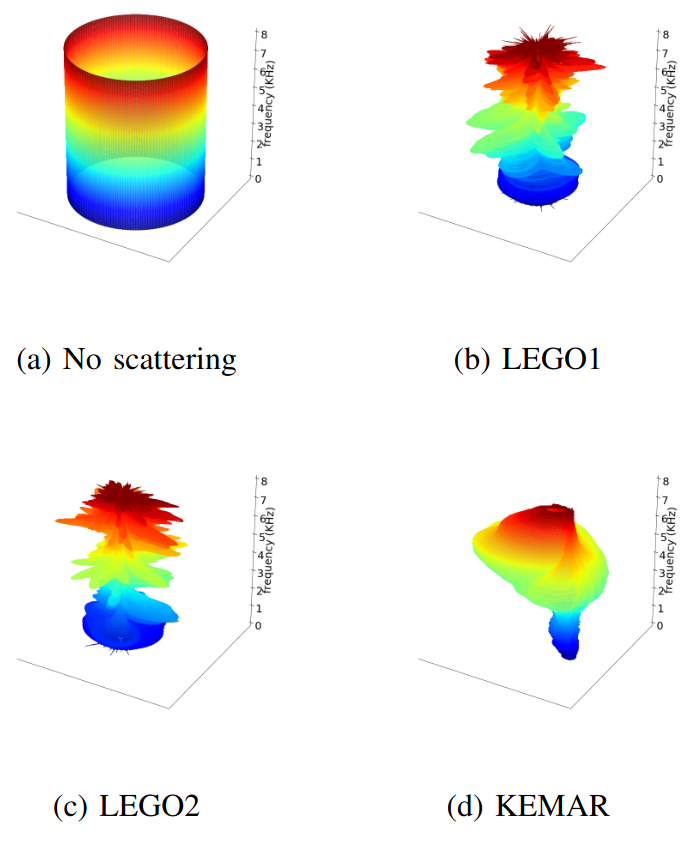
\includegraphics[scale = 0.35]{cones.png}
\caption{Directional frequency magnitude response for different devices. Each horizontal slice  corresponds to a frequency between 0-8000 Hz from bottom to top. These magnitudes doesn't correspond to our scatterings but can be used as illustrations for information. They correspond to the impulse responses of the paper \cite{dalia} from which the image comes from. These scatterings are comparable to ours.}
\label{fig:cones}
\end{figure}

In figure \ref{fig:cones} we can see different scatterings and the directional frequency magnitude response that is obtained with the respective scattering. Figure \ref{fig:cones}(a) illustrates the usual omnidirectional case and this image shows that localization without scattering is impossible when using only one microphone (i.e. monaural localization) as it has no proper asperities. Meaning that the condition $C_{J_1} = C_{J_2}$ implies  $J_1 = J_2$ doesn't hold at all. Figures \ref{fig:cones}(b) and \ref{fig:cones}(c) are magnitudes produced from LEGO scatterings that are comparable to the one that we have. Finally figure \ref{fig:cones}(d) is produced by a KEMAR head and is exactly corresponding to what we have for our KEMAR impulse responses meaning that it corresponds to a usual HRTF. It is easy to notice that the KEMAR scattering is smoother than the LEGO ones, probably because the head produces a weaker scattering than a lot of different LEGOs. Meaning that the LEGO scatterings will probably be the better ones here.

\subsubsection{Algorithm}

We can see the pseudo-code in the algorithm \ref{alg:stacking}. In the algorithm we compute the empirical PSD of y which is a sufficiently good approximation \cite{dalia}\cite{Ledoux}. Then, instead of comparing to the cones we compare to its smallest enclosing subspace $S_J = span \{|H_j|^2\}_{j \in J}$ represented by the following matrix 

\begin{equation}
    B_J = [|H_{j_1}|^2, |H_{j_2}|^2 ... |H_{j_L}|^2], j_k \in J.
\end{equation}

Meaning that selecting the closest cone can now be approximately determined by selecting the subspace projection of $J \subseteq D$ that has the smallest error. Of course this algorithm is only robust if there is enough difference in these projections meaning that if the angles are too close or if the scattering gives transfer functions that only vary smoothly across directions then the algorithm will not give as good results as it could because the subspaces would be too similar \cite{dalia}.

\begin{algorithm}[H]
\caption{White noise localization using scattering and stacking}\label{alg:stacking}
  \KwIn{Number of sources L, magnitudes of transfer functions \{$|H_j|^2$\}$_{j \in D}$, N audio frames $Y \in \mathbb{C}^{FxN}$ }
  \KwOut{Directions of arrival $\hat \Theta = \{ \hat \theta _1, \hat \theta _2, \hat \theta _3 ... \hat \theta _L \}$}
  Stack the transfer functions of the different microphones by appending them (HStack)
  
  Stack the observed signal of the different microphones by appending them (YStack)
  
  Compute the empirical PSD y = $\frac{1}{N} \sum_{n=1}^N |Y_n|^2$
    
    \For{every $ J  \subseteq D $, |J| = L}{
    $B_J \gets [|H_j|^2]_{j \in J}$
    \\$P_J \gets B_JB_J^\dag$
    }
    $\hat J \gets  argmin_J ||(I - P_J)y||$
    \\$\hat \Theta \gets \{\theta _j | j \in \hat J\} $
\end{algorithm}
